\documentclass[11pt]{article}
%autocompile publish
\usepackage{math-hse,array,tikz,amsfonts}
\usetikzlibrary{hobby,decorations.pathreplacing,arrows.meta}
\title{Лекция 1. Основные понятия теории вероятностей}

\date{13.01.2026}
\begin{document}
\section{Основные понятия}

\paragraph{Случайный эксперимент} Фундаментальное понятие теории вероятностей~--- случайный эксперимент. Это способ получить информацию, когда результат заранее не известен. Например: я брошу игральную кость~--- что на ней выпадет? Запишем, как человек произносит слово <<левиоса>>,~--- какой будет длина гласной <<о>>? Выйдем на улицу 15 января 2050 года~--- какой будет температура воздуха? В этих ситуациях бросок кости, запись слова у конкретного человека, замер температуры воздуха можно считать случайными экспериментами. Результат случайного эксперимента называется \emph{элементарным исходом}.

\paragraph{Множество элементарных исходов}  Множество всех возможных результатов случайного эксперимента будем называть \emph{множеством элементарных исходов}, или \emph{пространством элементарных исходов}. Обычно оно обозначается буквой $\Omega$.

\begin{examples}
\item[]
\begin{enumerate}
	\item Если мы бросаем кубик, то пространством элементарных исходов можно считать числа от 1 до 6.

	\item Если мы обсуждаем температуру 15 января 2050 года, то пространством элементарных исходов можно считать числа от --100 до +100.

	\item Исходом случайного испытания необязательно должно быть число. Что выпадет при бросании монетки: орёл или решка? На кого из ребят падёт жребий водить в игре: на~Саню, Петю, Митю или Лену?
\end{enumerate}
\end{examples}

Важно заметить, что во множество элементарных исходов входят только те исходы, которые нас интересуют: например, если мы бросаем кубик и хотим узнать, какое значение оказалось на верхней грани, мы не будем считать элементарным исходом событие <<прибежала собака и съела кубик>>. Это называется математическим моделированием.

\paragraph{События} \emph{Событием} мы будем называть любое подмножество множества элементарных исходов. События образуют \emph{алгебру событий}, которая обозначается буквой $\mathcal{A}$.

\paragraph{Благоприятные исходы} Если элементарный исход принадлежит какому-то событию, этот элементарный исход называется \emph{благоприятным} для этого события.

\begin{examples}
\item[]
\begin{enumerate}
	\item Случайный эксперимент: бросаем шестигранный кубик.
	
	Множество элементарных исходов $\Omega: \left\{1,2,3,4,5,6\right\}$.
	
	Событие $A$: на кубике выпало чётное число.
	
	Множество элементарных исходов, благоприятных событию $A$: $\left\{2,4,6\right\}$.
	
	\item Случайный эксперимент: измеряем температуру на улице 15 января 2050 года.
	
	Множество элементарных исходов $\Omega: \left\{\left[-100;100\right]\right\}$
	
	Событие $B$: на улице 15 января 2050 года холодно.
	
	Множество элементарных исходов, благоприятных событию $B$: $\left\{\left[-100;-5\right]\right\}$.
	
	$-20$~--- благоприятный исход для события $B$, $+10$~--- неблагоприятный.
	
	\item Случайный эксперимент: троекратное бросание монетки.
	
	Событие $C$: выпало хотя бы два орла. 
	
	Элементарный исход <<орёл, решка, орёл>> благоприятствует событию $C$, а элементарный исход <<решка, решка, орёл>> не благоприятствует событию $C$.
\end{enumerate}
\end{examples}

\paragraph{}Вспомним теорию множеств, чтобы было удобно описывать отношения между событиями.

\paragraph{Несовместные события} Если два события не могут произойти одновременно, они называются \emph{несовместными}. На языке теории множеств: пересечение двух событий~--- пустое множество.

\begin{center}
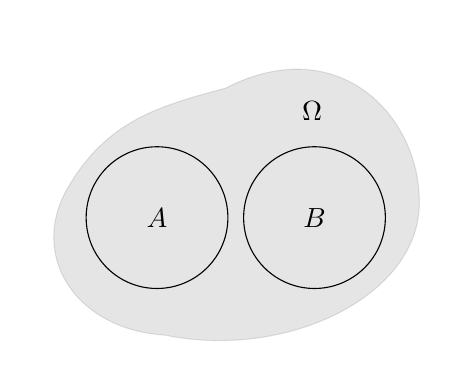
\begin{tikzpicture}
	
	\draw (-0.5,0) circle [radius=0.9cm];
	\node at (-0.5,0) {$A$};
	\draw (1.5,0) circle [radius=0.9cm];
	\node at (1.5,0) {$B$};
	\coordinate (C) at (0,0);
	\coordinate (D) at (1,0);
	
	\begin{scope}[rotate around={150:(0.4,0.7)}]
		\draw[fill = black, opacity = 0.1] (0.9,-0.1) .. controls (1.5,0.5) and (2,1) .. (2,2) .. controls (2,3) and (1,3.5) .. (0,3) .. controls (-1.5,2.5) and (-2.5,1) .. (-2,0) .. controls (-1.5,-1) and (0,-1.5) .. cycle;
		\node at (-0.2, -0.4) {$\Omega$};
	\end{scope}
\end{tikzpicture}
\end{center}

\begin{examples}
\item[]
\begin{enumerate}
	\item Случайный эксперимент: бросок шестигранного кубика.
	
	Событие $A$: выпало чётное число.
	
	Событие $B$: выпало число, меньшее трёх.
	
	События $A$ и $B$ совместны, т.\,к. элементарный исход <<выпадение двойки>> благоприятен для обоих событий. 
	
	Заметим, что не все элементарные исходы, благоприятные $A$, благоприятны и $B$: скажем, элементарный исход <<выпадение четвёрки>> благоприятен событию $A$, но не благоприятен $B$.

	\item Случайный эксперимент: троекратное бросание монетки.
	
	Событие $A$: выпало хотя бы два орла.
	
	Событие $B$: выпала хотя бы одна решка.
	
	Событие $C$: количество выпавших решек больше, чем количество выпавших орлов.
	
	События $A$ и $B$ совместны: элементарный исход <<решка, орёл, орёл>> благоприятствует обоим событиям. События $A$ и $C$ несовместны.
\end{enumerate}
\end{examples}

\newpage

\paragraph{Пересечение событий} Пусть $A$ и $B$~--- некоторые события. Событие $C$, состоящее в том, что выполняются события $A$ и $B$, мы будем называть \emph{пересечением} событий $A$ и $B$ и обозначать $A\cap B$. Ниже на диаграмме Эйлера\,---\,Венна пересечение событий $A$ и $B$ закрашено фиолетовым.

\begin{center}
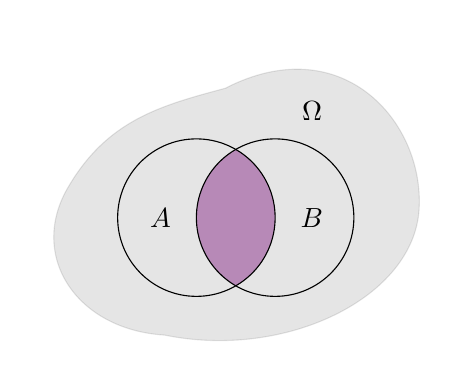
\begin{tikzpicture}
	
	\coordinate (A) at (0,0);
	\coordinate (B) at (1,0);
	\def\r{1cm}
	
	\begin{scope}
		\clip (A) circle (\r);                 
		\fill[violet, opacity=0.4] (B) circle (\r);
	\end{scope}
	
	\draw (A) circle (\r);
	\draw (B) circle (\r);	
	
	\node[left]  at (-0.2,0) {$A$};
	\node[right] at (1.2,0)   {$B$};
	
	
	\begin{scope}[rotate around={150:(0.4,0.7)}]
		\draw[fill = black, opacity = 0.1] (0.9,-0.1) .. controls (1.5,0.5) and (2,1) .. (2,2) .. controls (2,3) and (1,3.5) .. (0,3) .. controls (-1.5,2.5) and (-2.5,1) .. (-2,0) .. controls (-1.5,-1) and (0,-1.5) .. cycle;
		\node at (-0.2, -0.4) {$\Omega$};
	\end{scope}
	
\end{tikzpicture}
\end{center}

\begin{examples}
\item[]
\begin{enumerate}
	\item Случайный эксперимент: бросок игральной кости.
	
	Событие $A$: выпало чётное число.
	
	Событие $B$: выпало число, меньшее трёх.
	
	Событие $A\cap B$: выпало чётное число, меньшее трёх, т.\,е.~выпала двойка.

	\item Случайный эксперимент: троекратное бросание монетки.
	
	Событие $A$: выпало хотя бы два орла.
	
	Событие $B$: выпала хотя бы одна решка.
	
	Событие $A\cap B$ состоит в выпадении двух орлов и одной решки, ему благоприятны следующие элементарные исходы: <<орёл, орёл, решка>>, <<орёл, решка, орёл>> и <<решка, орёл, орёл>>.
\end{enumerate}
\end{examples}

\paragraph{Объединение событий} Пусть $A$ и $B$~--- некоторые события. Событие $C$, состоящее в том, что выполняются события $A$ или $B$ (можно оба сразу), мы будем называть \emph{объединением} событий $A$ и $B$ и обозначать $A\cup B$.

\begin{center}
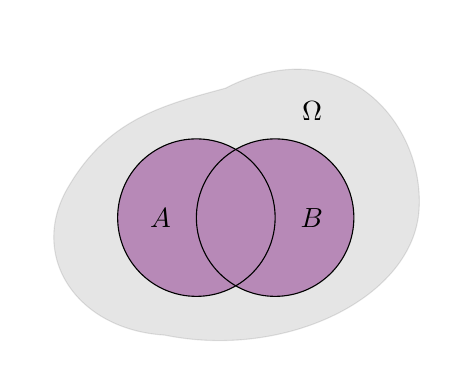
\begin{tikzpicture}
	
	\coordinate (A) at (0,0);
	\coordinate (B) at (1,0);
	\def\r{1cm}
	
	\begin{scope}
		\clip (A) circle (\r);
		\fill[violet, opacity=0.4, even odd rule] 
		(A) circle (\r) (B) circle (\r);
	\end{scope}
	\fill[violet, opacity=0.4] (B) circle (\r);
	
	% Перерисуем контуры поверх заливки, чтобы границы были чёткими
	\draw (A) circle (\r);
	\draw (B) circle (\r);	
	
	\node[left]  at (-0.2,0) {$A$};
	\node[right] at (1.2,0)   {$B$};
	
	
	\begin{scope}[rotate around={150:(0.4,0.7)}]
		\draw[fill = black, opacity = 0.1] (0.9,-0.1) .. controls (1.5,0.5) and (2,1) .. (2,2) .. controls (2,3) and (1,3.5) .. (0,3) .. controls (-1.5,2.5) and (-2.5,1) .. (-2,0) .. controls (-1.5,-1) and (0,-1.5) .. cycle;
		\node at (-0.2, -0.4) {$\Omega$};
	\end{scope}
	
\end{tikzpicture}
\end{center}

\paragraph{Дополнение к событию} Пусть $A$ ~--- некоторое событие. Событие $C$, состоящее в том, что событие $A$ не выполняется, мы будем называть \emph{дополнением} к событию $A$ и обозначать $\overline{A}$. Ниже на диаграмме Эйлера\,---\,Венна дополнение к событию $A$ закрашено фиолетовым.

\begin{center}
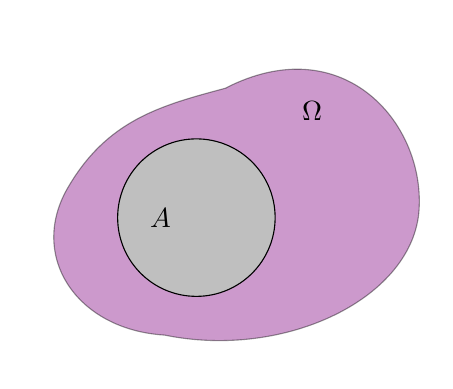
\begin{tikzpicture}
	\begin{scope}[rotate around={150:(0.4,0.7)}]
		\draw[fill = violet, opacity=0.4] (0.9,-0.1) .. controls (1.5,0.5) and (2,1) .. (2,2) .. controls (2,3) and (1,3.5) .. (0,3) .. controls (-1.5,2.5) and (-2.5,1) .. (-2,0) .. controls (-1.5,-1) and (0,-1.5) .. cycle;
		\node at (-0.2, -0.4) {$\Omega$};
	\end{scope}

	\coordinate (A) at (0,0);
	\def\r{1cm}
	
	\fill[fill = lightgray] (A) circle (\r);
	
	\draw (A) circle (\r);
	
	\node[left]  at (-0.2,0) {$A$};
\end{tikzpicture}
\end{center}

\paragraph{Вероятность события} Третьим элементов вероятностного пространства $(\Omega, \mathcal{A}, P)$ является функция вероятности $P$. Формально это функция, которая каждому элементарному исходу ставит в соответствие вещественное число от $0$ до $1$. При этом должны выполняться естественные свойства связанные с операция (пересечение, объединение, дополнение) в алгебре событий. Мы не будем разбирать подробно аксиоматическую теорию вероятности а ограничимся одной картинкой.

На рисунке ниже синие точки~--- элементарные исходы, $\Omega$~--- пространство элементарных исходов; красные эллипсы~--- события, $\mathcal{A}$~--- алгебра событий. Каждому событию соответствует значение вероятности $P$ от 0 до 1.

\begin{center}
	\resizebox{0.7\textwidth}{!}{%
		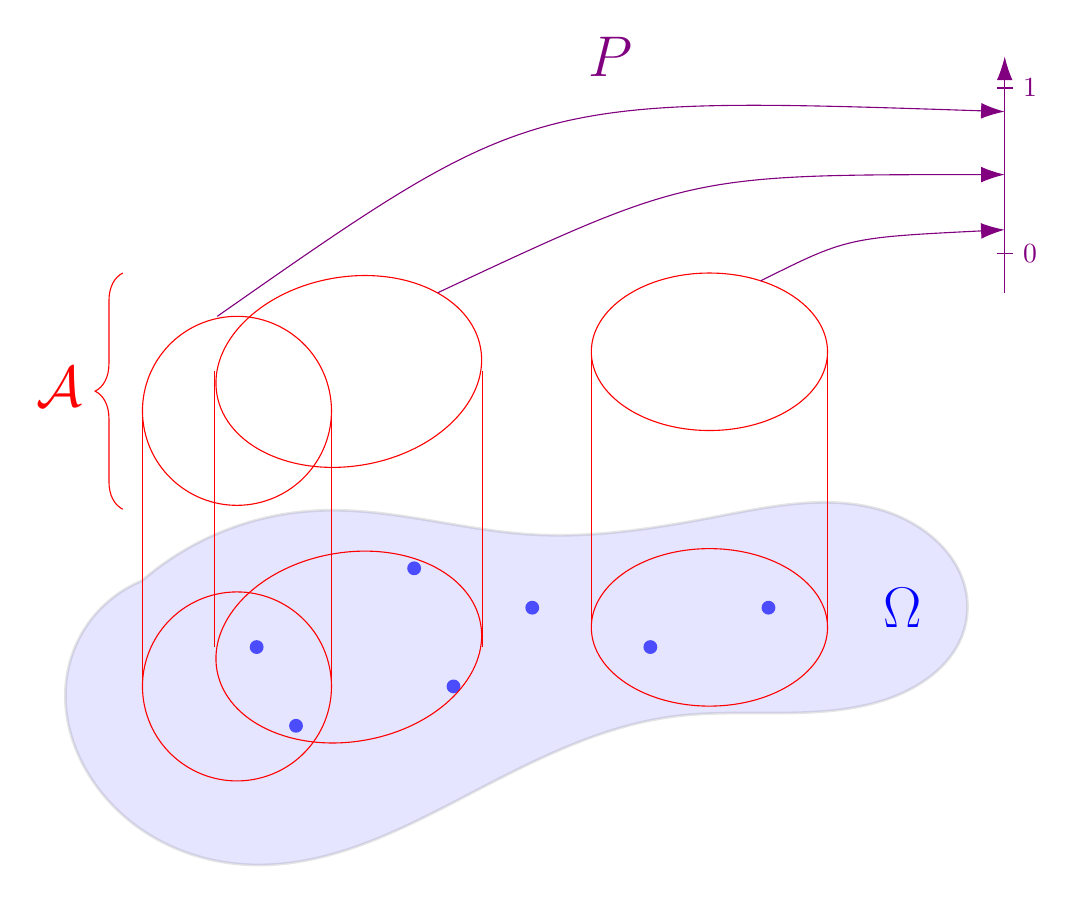
\begin{tikzpicture}[>={Latex[length=3mm,width=2mm]}, line width=1pt] % В квадратных скобках увеличение размера стрелочек
			%======================
			% Параметры цвета и размера
			%======================
			\def\fillColor{blue!70}       % Цвет для точек
			\def\fillOpacity{0.1}         % Прозрачность заливки множества
			\def\pointRadius{2.5pt}         % Радиус точек
			\def\redLineWidth{thin}       % Толщина красных линий
			\def\greenLineWidth{thin}    % Толщина зеленых линий
			\def\violetLineWidth{thin}   % Толщина фиолетовых линий
			\def\braceAmplitude{10pt}     % Амплитуда скобки
			
			%======================
			% Контур множества Ω
			%======================
			\draw[fill=blue, opacity=\fillOpacity, use Hobby shortcut] 
			(2.04,3.84)
			.. (4.22,4.73)
			.. (6.99,4.43)
			.. (9.36,4.66)
			.. (11.4,4.75)
			.. (12.52,3.39)
			.. (11.42,2.31)
			.. (8.81,2.12)
			.. (6.14,1.10)
			.. (3.32,0.24)
			.. (1.38,1.36)
			.. (1.12,2.78)
			.. (2.04,3.84);
			
			%======================
			% Координаты точек
			%======================
			\coordinate (P1) at (3.5,3.0);
			\coordinate (P2) at (5.5,4.0);
			\coordinate (P3) at (7.0,3.5);
			\coordinate (P4) at (8.5,3.0);
			\coordinate (P5) at (10.0,3.5);
			\coordinate (P6) at (6.0,2.5);
			\coordinate (P7) at (4.0,2.0);
			
			%======================
			% Отрисовка точек
			%======================
			\foreach \p in {P1,P2,P3,P4,P5,P6,P7} {
				\fill[\fillColor] (\p) circle (\pointRadius);
			}
			
			%======================
			% Красные эллипсы и вертикальные линии
			% Формат: x/y/radiusX/radiusY/angle/lineHeight
			% lineHeight - высота линии до верхнего эллипса в колонке
			%======================
			\foreach \x/\y/\rx/\ry/\angle/\lineH in {
				3.25/2.5/1.2/1.2/15/3.5,   % нижний эллипс левой колонки
				3.25/6.0/1.2/1.2/15/0,     % верхний эллипс левой колонки
				9.25/3.25/1.5/1.0/0/3.5,   % нижний эллипс правой колонки
				9.25/6.75/1.5/1.0/0/0,     % верхний эллипс правой колонки
				4.67/3.0/1.7/1.2/10/3.5,   % нижний эллипс центральной колонки
				4.67/6.5/1.7/1.2/10/0      % верхний эллипс центральной колонки
			} {
				% Эллипс
				\draw[red,\redLineWidth,rotate around={\angle:(\x,\y)}] (\x,\y) ellipse (\rx cm and \ry cm);
				% Вертикальные линии
				\ifdim \lineH pt>0pt
				\draw[red,\redLineWidth] (\x-\rx,\y) -- ++(0,\lineH);
				\draw[red,\redLineWidth] (\x+\rx,\y) -- ++(0,\lineH);
				\fi
			}
			
			% Красная скобка
			\draw[red,\redLineWidth,decorate,decoration={brace, amplitude=\braceAmplitude}] 
			(1.8,4.75) -- (1.8,7.75);
			
			% Подписи множеств
			\node[red] at (1,6.3) {\huge $\mathcal{A}$};
			\node[blue] at (11.7,3.5) {\huge $\Omega$};
			
			%======================
			% Зелёные стрелки (ξ)
			%======================
			%		\draw[green,\greenLineWidth,->] (13,-1.5) -- ++(0,3); % ось ξ
			%		\draw[green,\greenLineWidth,->] (P3) .. controls (9, -0.3) .. (13,0.3);
			%		\draw[green,\greenLineWidth,->] (P4) .. controls (10, 0.4) .. (13,1);
			%		\draw[green,\greenLineWidth,->] (P7) .. controls (7, -1.0) .. (13,-0.6);
			%		\node[green] at (9,-1.3) {\huge $\xi$};
			%		\node[green] at (13.5,1) {\huge $\mathbb{R}$};
			
			%======================
			% Фиолетовые стрелки (P)
			%======================
			\draw[violet,\violetLineWidth,->] (13,7.5) -- ++(0,3); % ось P
			\draw[violet,\violetLineWidth,->] (3,7.2) .. controls (7,10) .. (13,9.8);
			\draw[violet,\violetLineWidth,->] (5.8,7.5) .. controls (9,9) .. (13,9);
			\draw[violet,\violetLineWidth,->] (9.9,7.65) .. controls (11,8.2) .. (13,8.3);
			
			% Засечки на оси P
			\draw[violet,\violetLineWidth] (12.9,8) -- (13.1,8);
			\draw[violet,\violetLineWidth] (12.9,10.1) -- (13.1,10.1);
			\node[violet,anchor=west] at (13.1,8) {0};
			\node[violet,anchor=west] at (13.1,10.1) {1};
			\node[violet] at (8,10.5) {\huge $P$};
			
		\end{tikzpicture}
	}
\end{center}

Обратите внимание: \textbf{вероятность не может быть отрицательной и не может быть больше единицы}!

\paragraph{Классическая схема вероятности} Рассмотрим такую ситуацию, в которой все исходы <<равноправны>>, то есть встречаются одинаково часто, если повторять эксперимент много раз. Такие исходы называют \emph{равновероятными}. Скажем, элементарные исходы <<1>>, <<2>>, <<3>>, <<4>>, <<5>>, <<6>> при бросании игральной кости естественно считать равновероятными (если, конечно, кость не кривая), а вот в случайном испытании <<Встречу ли я динозавра, выходя сегодня из дверей университета?>> исходы <<да>> и <<нет>> равновероятными не являются. Путь, кроме того, общее количество исходов конечно (это довольно частый случай, например с кубиком, монеткой, рулеткой). В этом случае такую модель называют \emph{классической схемой вероятности}, а функция вероятности задаётся явным образом.

\paragraph{Вероятность события в классической схеме} \emph{Вероятностью события A} в классической схеме вероятности, мы будем называть отношение количества элементарных исходов, благоприятных событию $A$ к общему количеству элементарных исходов:
$$
	P(A)=\frac{N(A)}{N(\Omega)}
$$



\begin{examples}
	\item Найдём вероятность выпадения чётного числа на игральной кости: $P(A)=N(A)/N(\Omega)=3/6=1/2$, т.~к. на игральной кости всего три чётных числа: ~2, ~4, ~6.

	\item Найдём вероятность выпадения хотя бы одной решки при троекратном бросании монетки.

Вот все возможные исходы, их восемь:

   <<орёл, орёл, орёл>>

   <<орёл, орёл, решка>>

   <<орёл, решка, орёл>>

   <<орёл, решка, решка>>

   <<решка, орёл, орёл>>

   <<решка, орёл, решка>>

   <<решка, решка, орёл>>

   <<решка, решка, решка>>

Событию <<выпала хотя бы одна решка>> благоприятны семь исходов~--- все, кроме первого. Итак, искомая вероятность:
$P(A)=N(A)/N(\Omega)=7/8$.
\end{examples}

Заметим, что \emph{сумма вероятностей всех элементарных исходов случайного эксперимента равна единице}:
$$
	N(\Omega)\times\frac{1}{N(\Omega)}=1.
$$

\begin{examples}
Случайный эксперимент: кидаем игральную кость. Имеем шесть возможных элементарных исходов, вероятность каждого $1/6$, сумма вероятностей равна 1.
\end{examples}

\paragraph{Достоверное событие} Если какому-то событию принадлежат все элементарные исходы (т.\,е.~событие совпадает с пространством элементарных исходов), то такое событие называется \emph{достоверным}. $P(\Omega)=1$.

\paragraph{Невозможное событие} Если нет ни одного элементарного исхода, благоприятного событию, то такое событие называется \emph{невозможным}. $P(\varnothing)=0$.

\section{Классическая схема вероятностей}
\begin{enumerate}
	\item Пространство элементарных исходов конечно:
	
	$$
	|\Omega|<\infty.
	$$
	
	\emph{(Напомним, что $|\Omega|$~--- это обозначение мощности множества $\Omega$, т.\,е.~количества элементов множества $\Omega$.)}
	
	\item Все элементарные исходы равновероятны:
	$$
	P(A)=\frac{|A|}{|\Omega|}.
	$$
	
\end{enumerate}

\section{Геометрическая схема вероятностей}
\begin{enumerate}
	\item Пространство элементарных исходов~--- часть n-мерного пространства действительных чисел $\mathbb{R}^n$ (при $n=2$ это плоскость, при $n=3$~--- трёхмерное пространство):
	
	$$
	\Omega\in\mathbb{R}^n.
	$$
	
	\item Элементарные исходы~--- точки в этом пространстве. Они равновероятны.
	
	\emph{Вероятность попасть в конкретную точку равна нулю}.
	$$
	P(A)=\frac{\mu(A)}{\mu(\Omega)}.
	$$
	
	$\mu$~--- это мера. В одномерном пространстве это длина, в двумерном~--- площадь, в~трёхмерном~--- объём, в четырёхмерном~--- четырёхмерный объём.
	
\end{enumerate}

\newpage

\begin{examples}
	Представьте, что вы стреляете из арбалета. Вы кладёте болт на ложе и целитесь в мишень — какова вероятность попасть в яблочко?
	
\begin{center}
	\resizebox{0.4\textwidth}{!}{%
	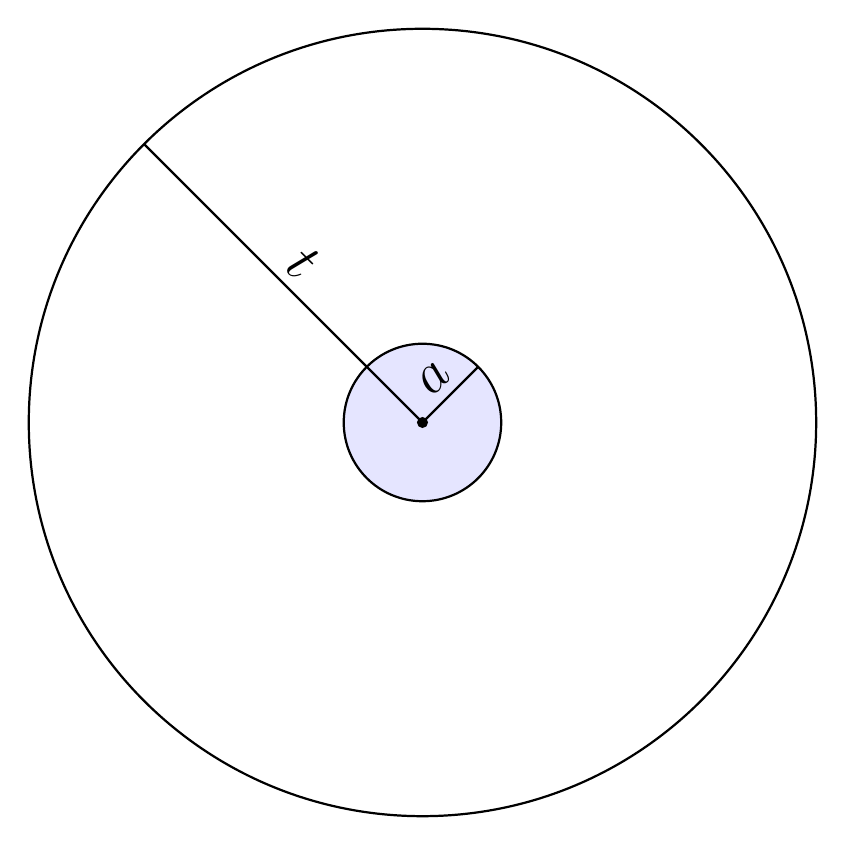
\begin{tikzpicture}
		% Мишень радиуса 5
		\draw[thick] (0,0) circle (5);
		
		% Яблочко радиуса 1
		\fill[blue!20, opacity=0.5] (0,0) circle (1);
		\draw[thick] (0,0) circle (1);
		
		% Радиус яблочка (45 градусов)
		\draw[thick] (0,0) -- ({cos(45)},{sin(45)})
		node[pos=0.5, rotate=45, above] {\huge$a$};
		
		% Радиус мишени (135 градусов)
		\draw[thick] (0,0) -- ({5*cos(135)},{5*sin(135)})
		node[pos=0.5, rotate=315, above] {\huge$t$};
		
		% Центр
		\fill (0,0) circle (2pt);
	\end{tikzpicture}
	}
\end{center}
	
	Мишень плоская, поэтому мера $\mu$ в данном случае~--- площадь поверхности.
	
	Пусть радиус «яблочка» $a=1$, радиус всей мишени $t=5$. Событие «вы попали в~яблочко» обозначим буквой $A$. По формуле площади круга:
	
	$$
	P(A)=\frac{S(A)}{S(\Omega)}=\frac{\pi{a}^2}{\pi{t}^2} =\frac{1^2}{5^2}=\frac{1}{25}.
	$$
\end{examples}

\paragraph{Дополнительные события} Мы будем говорить, что события $A$ и $B$ являются \emph{дополнительными}, если $A$ и $B$ вместе составляют всё пространство элементарных исходов $\Omega$ и~являются несовместными. Дополнение к событию $A$ обозначают $B=\overline{A}$.

\begin{examples}
	События $A$~--- на игральной кости выпало чётное число  и $B$~--- на игральной кости выпало нечётное число~--- являются дополнительными: действительно, каждое выпавшее на игральной кости число будет обязательно или чётным, или нечётным.
\end{examples}

\emph{Сумма вероятностей дополнительных событий равна единице}:

$$
P(A)+P(\overline{A})=1.
$$

\begin{examples}
   \item Пусть события $A$~--- на игральной кости выпало чётное число и $B$~--- на игральной кости выпало нечётное число. Тогда $P(A)=3/6=1/2$, т.\,к. ~событию $A$ благоприятны три исхода: выпадение <<2>>, <<4>> или <<6>>; $P(B)=3/6=1/2$, т.\,к. ~событию $B$ благоприятны три исхода: выпадение <<1>>, <<3>> или <<5>>. Сумма вероятностей $P(A)+P(B)=1/2+1/2=1$.\\

\end{examples}

В прошлый раз мы обсуждали связь между вероятностью и действием взятия дополнения к событию. Можно аналогичным образом написать формулу для связи вероятности и~объединения событий:

\begin{theorem*}
	[Теорема сложения вероятностей]
	Для любых двух событий $A$ и $B$ вероятность того, что хотя бы одно из событий произойдёт, равна сумме вероятностей событий $A$ и $B$ минус вероятность их одновременного выполнения:
	$$
	P(A\cup B)=P(A)+P(B)-P(A\cap B).
	$$
\end{theorem*}

Если представить это на диаграмме Эйлера\,---\,Венна, то можно заметить, что при сложении двух пересекающихся множеств их пересечение (фиолетовую область) мы посчитаем дважды~--- поэтому нужно вычесть пересечение $A$ и $B$.

\begin{center}
	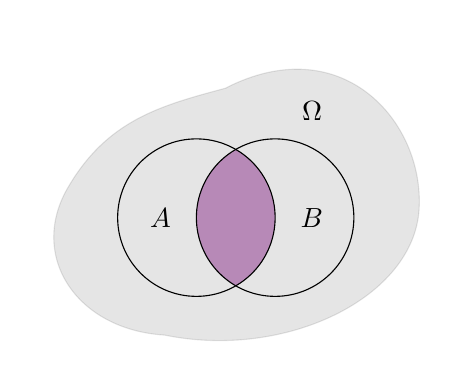
\begin{tikzpicture}
		
		\coordinate (A) at (0,0);
		\coordinate (B) at (1,0);
		\def\r{1cm}
		
		\begin{scope}
			\clip (A) circle (\r);                 
			\fill[violet, opacity=0.4] (B) circle (\r);
		\end{scope}
		
		\draw (A) circle (\r);
		\draw (B) circle (\r);	
		
		\node[left]  at (-0.2,0) {$A$};
		\node[right] at (1.2,0)   {$B$};
		
		
		\begin{scope}[rotate around={150:(0.4,0.7)}]
			\draw[fill = black, opacity = 0.1] (0.9,-0.1) .. controls (1.5,0.5) and (2,1) .. (2,2) .. controls (2,3) and (1,3.5) .. (0,3) .. controls (-1.5,2.5) and (-2.5,1) .. (-2,0) .. controls (-1.5,-1) and (0,-1.5) .. cycle;
			\node at (-0.2, -0.4) {$\Omega$};
		\end{scope}
		
	\end{tikzpicture}
\end{center}

\section{Условная вероятность}

\begin{definition}
	\emph{Условной вероятностью} $P(A|B)$ события $A$ при условии $B$ называется отношение вероятности пересечения $A\cap B$ к вероятности события $B$:
	$$
	P(A|B)=\frac{P(A\cap B)}{P(B)}.
	$$
	Если все элементарные исходы равновероятны, то эта вероятность равна отношению количества исходов, благоприятных обоим событиям, к количеству исходов, благоприятных событию $B$:
	$$
	P(A|B)=\frac{N(A\cap B)}{N(B)}.
	$$
\end{definition}

Рассмотрим ситуацию. Во дворе играют 20 детей: 12 мальчиков и 8 девочек (см.
табл.~\ref{deti}). Дети играют в футбол и в классики. В футбол играют 8 мальчиков и 2 девочки, в классики остальные ребята, т.\,е.~4 мальчика и 6 девочек. Выберем случайным образом ребёнка среди играющих. С какой вероятностью он играл в футбол? Ответ следует непосредственно из~определения вероятности:
$$
P(F)=\frac{N(F)}{N(\Omega)}=\frac{10}{20}=\frac{1}{2}.
$$

\begin{table}[b]
	\begin{center}
		\begin{tabular}{|c|c|c|c|c|}
			\hline
			& классики & футбол & всего \\
			\hline
			девочки & 6 & 2 & 8 \\
			\hline
			мальчики & 4 & 8 & 12 \\
			\hline
			всего & 10 & 10 & 20 \\
			\hline
		\end{tabular}
		\caption{Дети во дворе}\label{deti}
	\end{center}
\end{table}
Теперь представим себе, что мы видим: выбранный случайным образом ребёнок оказался мальчиком. С какой вероятностью он играл в футбол? Теперь изменилось и количество благоприятных исходов, и общее количество исходов.
$$
P(F|M)=\frac{N(F\cap M)}{N(M)}=\frac{8}{12}=\frac{2}{3},
$$
где $P(F|M)$~--- вероятность того, что выбранный ребёнок играет в футбол, при условии, что он оказался мальчиком, $n(F\cap M)$~--- количество мальчиков играющих в футбол, $n(M)$~--- общее количество мальчиков. Посмотрим на наше вычисление внимательнее:
$$
P(F|M)=\frac{\frac{N(F\cap M)}{N(\Omega)}}{\frac{N(M)}{N(\Omega)}}=\frac{P(F\cap M)}{P(M)}.
$$

Здесь $P(F\cap M)$~--- вероятность того, что случайно взятый ребёнок оказался мальчиком, играющим в футбол, $P(M)$~--- вероятность того, что случайно взятый ребёнок оказался мальчиком. Эту формулу можно воспринимать как определение \emph{условной вероятности}: вероятностью события $A$ при условии $B$ называется отношение вероятности их одновременного выполнения к вероятности события $B$.

Важно не путать два понятия: вероятность одновременного выполнения двух событий и~вероятность события $A$ при условии $B$. Можно считать, что во втором случае мы рассматриваем не все элементарные исходы, а только те, что благоприятны $B$.

\begin{example}
	При бросании игральной кости события $A$~--- выпадение чётного числа  и $B$~--- выпадение числа, меньшего трёх. Найдём вероятность события $A$ при условии $B$, т.\,е.~вероятность выпадения чётного числа, при условии, что выпало меньше трех. Мы уже выяснили, что событие $AB$ состоит в выпадении двойки, т.\,е.~$P(A\cap B)=1/6$,~ $P(B)=2/6=1/3$, тогда
	$$
	P(A|B) =\frac{P(A\cap B)}{P(B)}=\frac{1/6}{1/3}=\frac{1}{2}.
	$$
\end{example}
\begin{example}
	Случайное испытание: троекратное бросание монетки. Случайное событие $A$~--- выпадение хотя бы двух орлов и $B$~--- выпадение хотя бы одной решки. Найдём вероятность события $A$ при условии $B$, выпадение хотя бы двух орлов при условии выпадение хотя бы одной решки. Мы уже выяснили, что событию $A\cap B$ благоприятствуют три элементарных исхода: «орёл, орёл, решка», «орёл, решка, орёл», «решка, орёл, орёл». Значит, $P(A\cap B)=3/8$, $P(B)=7/8$. Итак:
	$$
	P(A|B) =\frac{P(A\cap B)}{P(B)}=\frac{3/8}{7/8}=\frac{3}{7}.
	$$
\end{example}

\begin{example}
	Рассмотрим ситуацию: вы кидали монетку уже 3 раза, и каждый раз выпадал орёл. С какой вероятностью и на четвёртый раз снова выпадет орёл? Орёл четыре раза подряд выпадает достаточно редко, значит, сейчас скорее выпадет решка, чем орёл, подсказывает нам интуиция. И ошибается! Действительно, вероятность события «выпали четыре решки подряд» составляет $1/16$, т.\,е. достаточно мала. Здесь благоприятным является единственный из 16 возможных исходов: РРРР, ОРРР, РОРР, РРОР, РРРО, ООРР, ОРОР, ОРРО, РООР, РОРО, РРОО, ОООР, ООРО, ОРОО, РООО, ОООО. Условная же вероятность события «в четвёртый раз выпала решка», при условии «первые три раза выпадала решка»  составит $1/2$, т.\,к. ~есть всего два равноправных исхода, в которых первые три раза выпадала решка. Здесь именно выполнение условия является редким событием, а~не выпадение решки при условии уже выпавших трёх.
\end{example}

\section{(Не)зависимость событий}

\begin{theorem*}[Теорема умножения вероятностей]
	Вероятность пересечения событий равна произведению условной вероятности на вероятность условия:
	$$
	P(A\cap B)=P(A|B)P(B).
	$$
\end{theorem*}

События $A$ и $B$ называются \emph{независимыми}, если вероятность события $A$ не зависит от~того, произошло $B$ или нет. Формально: $P(A|B)=P(A)$.

\begin{example}
	Зависимы ли события «выбранный ребёнок играет в футбол» и «выбранный ребёнок~--- мальчик» из рассмотренного раньше примера?
	
	Как мы посчитали раньше (см. таблицу~\ref{deti}):
	
	$P(F)=10/20=1/2$,
	
	$P(F |M)=8/12=2/3$,
	
	$P(F)\neq P(F |M)$~--- значит, события не являются независимыми. Это означает, что доля футболистов среди мальчиков больше, чем доля футболистов среди всех детей.
\end{example}

\begin{example}
	Зависимы ли события: $A$~--- выпадение чётного числа при бросании игральной кости и $B$~--- выпадение числа, меньшего трёх?
	
	$P(A)=3/6$,
	
	$P(A|B)=1/2$,
	
	$P(A)= P(A|B)$~--- значит, события независимы. Это означает, что доля чётных чисел среди первых двух такая же, как и среди всех шести возможных.
\end{example}

Мы знаем, что: $P(A|B) =P(A\cap B)/P(B)$. Значит, условие независимости событий можно записать так: $P(A)=P(A|B)=P(A\cap B)/P(B)$. Откуда получаем:

$$P(A\cap B)=P(A)\times P(B).$$

Это важное свойство независимых событий, часто его берут за основное определение.

Иногда вопрос о зависимости двух событий можно рассматривать как математическую задачку, как мы делали выше. Бывают же ситуации когда, наоборот, из природы событий ясно, что они независимы, тогда их независимостью можно пользоваться для нахождения вероятности одновременного выполнения событий.

\begin{example}
	Монетку бросили три раза. С какой вероятностью выпало три решки? Эту задачу мы уже решили, подсчитав общее количество элементарных исходов и количество благоприятных исходов. Посмотрим теперь на этот вопрос следующим образом. Интересующее нас событие $A$ состоит в одновременном выполнении трёх событий: $B$~--- в первый раз выпала решка, $C$~--- во второй раз выпала решка, $D$~--- в третий раз выпала решка. Эти события независимы (если, конечно, мы не заинтересованы в результате и бросаем монетку честно). Значит,
	$$
	P(A)=P(B\cap C\cap D)=P(B)\times P(C)\times P(D)=\frac{1}{2}\times\frac{1}{2}\times\frac{1}{2}=\frac{1}{8}.
	$$
\end{example}

\begin{example}
	Монетку бросили три раза. Найти вероятность события $A$~--- выпал хотя бы один орёл. На первый взгляд, мы не можем применять в этой задаче соображения независимости событий, ведь «выпал хотя бы один орёл»~--- это значит, что мог выпасть именно один орёл в любой из разов, могло выпасть два орла, могло выпасть три орла, т.\,е.~само событие устроено сложно. В чем состоит дополнительное событие $B=\Omega \verb|\| A $? Другими словами, в~каких случаях событие A не выполняется? Когда не выпало ни одного орла, т.\,е.~выпали три решки. Вероятность этого события мы только что нашли: $P(B)=1/2\times1/2\times1/2=1/8$. Значит, $P(A)=1-P(B)=7/8$.
\end{example}

\end{document}
